%%----------------------------------------------------------------------------------------
%	PACKAGES AND THEMES
%----------------------------------------------------------------------------------------
\PassOptionsToPackage{table}{xcolor}
\documentclass[aspectratio=169,xcolor=dvipsnames,svgnames,x11names,fleqn]{beamer}
% \documentclass[aspectratio=169,xcolor=dvipsnames,fleqn]{beamer}

\usetheme{RedVelvet}

\usefonttheme[onlymath]{serif}
\newcommand{\showanswers}{yes}
\usepackage{pifont} % For checkmarks and crosses

\usepackage{setspace}
\usepackage{xspace}
\usepackage{amsmath}
\usepackage{amssymb}
\usepackage{amsfonts}
\usepackage{color}
\usepackage{physics}
% \usepackage{mathbb}
\usepackage{rahul_math}
\usepackage{bigints}

\usepackage{graphicx} % Allows including images
\usepackage{booktabs} % Allows the use of \toprule, \midrule and \bottomrule in tables
\usepackage{tikz,pgfplots}
\usepackage{mathtools}
\usepackage{subfigure}
\usetikzlibrary{arrows}
\usepackage{minted}
\definecolor{LightGray}{gray}{0.9}
\definecolor{cream}{rgb}{0.92, 0.9, 0.55}
\definecolor{lightblue}{rgb}{0.68, 0.85, 0.9}


\usepackage{xcolor-material}
\usetikzlibrary{fit}
\usetikzlibrary{matrix}
\tikzset{%
apple/.pic={
    \fill [MaterialBrown] (-1/8,0)  arc (180:120:1 and 3/2) coordinate [pos=3/5] (@)-- ++(1/6,-1/7)  arc (120:180:5/4 and 3/2) -- cycle;
    \fill [MaterialLightGreen500] (0,-9/10)  .. controls ++(180:1/8) and ++(  0:1/4) .. (-1/3,  -1) .. controls ++(180:1/3) and ++(270:1/2) .. (  -1,   0) .. controls ++( 90:1/3) and ++(180:1/3) .. (-1/2, 3/4) .. controls ++(  0:1/8) and ++(135:1/8) .. (   0, 4/7)
    }
    }

\newcommand{\leftdoublequote}{\textcolor{blue}{\scalebox{3}{``}}}

\newcommand{\rightdoublequote}{\textcolor{blue}{\scalebox{3}{''}}}


\usepackage{textcomp}
\usepackage{fontawesome}
\usepackage{tikz,pgfplots}
\usetikzlibrary{shapes.callouts}
\usetikzlibrary{arrows}
\usetikzlibrary{shapes.geometric, positioning}
\usetikzlibrary{matrix,positioning,decorations.pathreplacing,calc}
\usepackage{tikz-dependency}

\pgfplotsset{compat=1.8} % or newest version

\usetikzlibrary{positioning}


\usepackage{bm}
\usepackage{relsize}

\tcbuselibrary{skins, hooks}

\tikzset{basic/.style={draw,fill=MediumBlue!20,text width=1em,text badly centered}}
\tikzset{input/.style={basic,circle}}
\tikzset{weights/.style={basic,rectangle}}
\tikzset{functions/.style={basic,circle,fill=MediumBlue!10}}



\usepackage{listofitems} % for \readlist to create arrays
\tikzstyle{mynode}=[thick,draw=MediumBlue,fill=MediumBlue!20,circle,minimum size=22]


\usepackage{overpic}

%----------------------------------------------------------------------------------------
%	TITLE PAGE
%----------------------------------------------------------------------------------------

\usepackage{tikz-qtree,tikz-qtree-compat}
\usetikzlibrary{tikzmark}
\usetikzlibrary{calc}

\usetikzlibrary{fit}
\tikzset{%
apple/.pic={
    \fill [MaterialBrown] (-1/8,0)  arc (180:120:1 and 3/2) coordinate [pos=3/5] (@)-- ++(1/6,-1/7)  arc (120:180:5/4 and 3/2) -- cycle;
    \fill [MaterialLightGreen500] (0,-9/10)  .. controls ++(180:1/8) and ++(  0:1/4) .. (-1/3,  -1) .. controls ++(180:1/3) and ++(270:1/2) .. (  -1,   0) .. controls ++( 90:1/3) and ++(180:1/3) .. (-1/2, 3/4) .. controls ++(  0:1/8) and ++(135:1/8) .. (   0, 4/7)
}
}
\usepackage{tikz-qtree,tikz-qtree-compat}
\usetikzlibrary{tikzmark}
\usetikzlibrary{calc}

\usetikzlibrary{positioning}

% Define styles
\tikzset{
    box/.style={
        rectangle,
        draw=black,
        fill=blue!20,
        text width=2.2cm,
        text centered,
        minimum height=0.8cm,
        font=\small
    },
    arrow/.style={
        ->,
        >=Stealth,
        line width=1.5pt,
        draw=black
    }
}


\usepackage{bm}
\usepackage{relsize}



\tikzset{basic/.style={draw,fill=MediumBlue!20,text width=1em,text badly centered}}
\tikzset{input/.style={basic,circle}}
\tikzset{weights/.style={basic,rectangle}}
\tikzset{functions/.style={basic,circle,fill=MediumBlue!10}}
\usetikzlibrary{arrows.meta, bending}
\usetikzlibrary{shapes.geometric, arrows.meta, positioning, fit, backgrounds}

\usepackage{listofitems} % for \readlist to create arrays
\tikzstyle{mynode}=[thick,draw=MediumBlue,fill=MediumBlue!20,circle,minimum size=22]


\newmdenv[
backgroundcolor=androidYellowLight,
linecolor=androidYellow,
linewidth=0.5pt,
roundcorner=10pt,
skipabove=\baselineskip,
skipbelow=\baselineskip
]{MintedFrame}

% Set minted options
\setminted{
fontsize=\footnotesize,
breaklines=true,
autogobble,
linenos,
frame=none
}


\title[CPE 487/587: Deep Learning]{CPE 486/586: Deep Learning for Engineering Applications} % The short title appears at the bottom of every slide, the full title is only on the title page
\subtitle{06 Generative Adversarial Network}

\author[Rahul Bhadani] {{\Large \textbf{Rahul Bhadani}}}

\institute[UAH] % Your institution as it will appear on the bottom of every slide, maybe shorthand to save space
{
    Electrical \& Computer Engineering,  The University of Alabama in Huntsville
}
\date

% \titlegraphic{
%    \includegraphics[width=0.4\linewidth]{figures/UAH_primary.png}
% }

\begin{document}

%-------------------------------------------------
\begin{frame}
    \titlepage
\end{frame}

%-------------------------------------------------
\begin{frame}{Outline}
    \backgroundtableofcontents
\end{frame}

%------------------------------------------------
\begin{frame}{}
    \begin{center}
        \huge \bf \color{DarkBlue}
        Motivation 
    \end{center}
    \end{frame}
    

%------------------------------------------------
\begin{frame}{Lecture Overview}
    \begin{itemize}
        \item In this lecture we discussed generative models (briefly) and how to model distributions of data using density estimation techniques. One advantage to these generative models is that we can generate data from the distribution once we have the model.   
        \item Our goal in this lecture is to introduce {\em \color{MediumRed}Generative Adversarial Networks} (GANs) for generating data from a distribution $p_{data}(\x)$. GANs are able to model complex distributions of data that would be incredible challenging to model using the density estimation approaches discussed in previous lectures. 
        \item Modeling $p_{data}(\x)$ is increasingly challenging for complex data, such as real scenes, people, etc. 
    \end{itemize}
\end{frame}


%------------------------------------------------
\begin{frame}{Example of a Complex $p_{data}(\x)$ }
\begin{center}
\uncover<2->{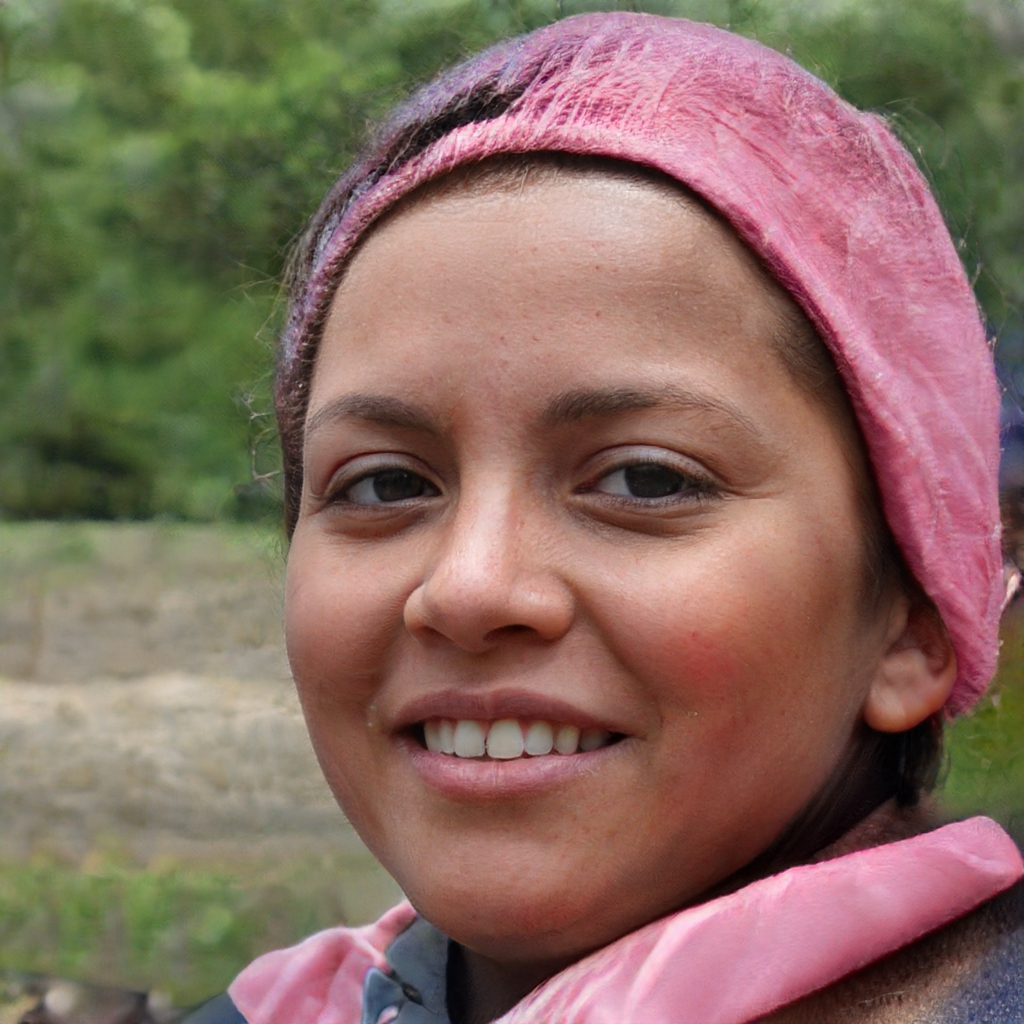
\includegraphics[width=.3\textwidth]{figures/gan-p1.jpg}}
\uncover<3->{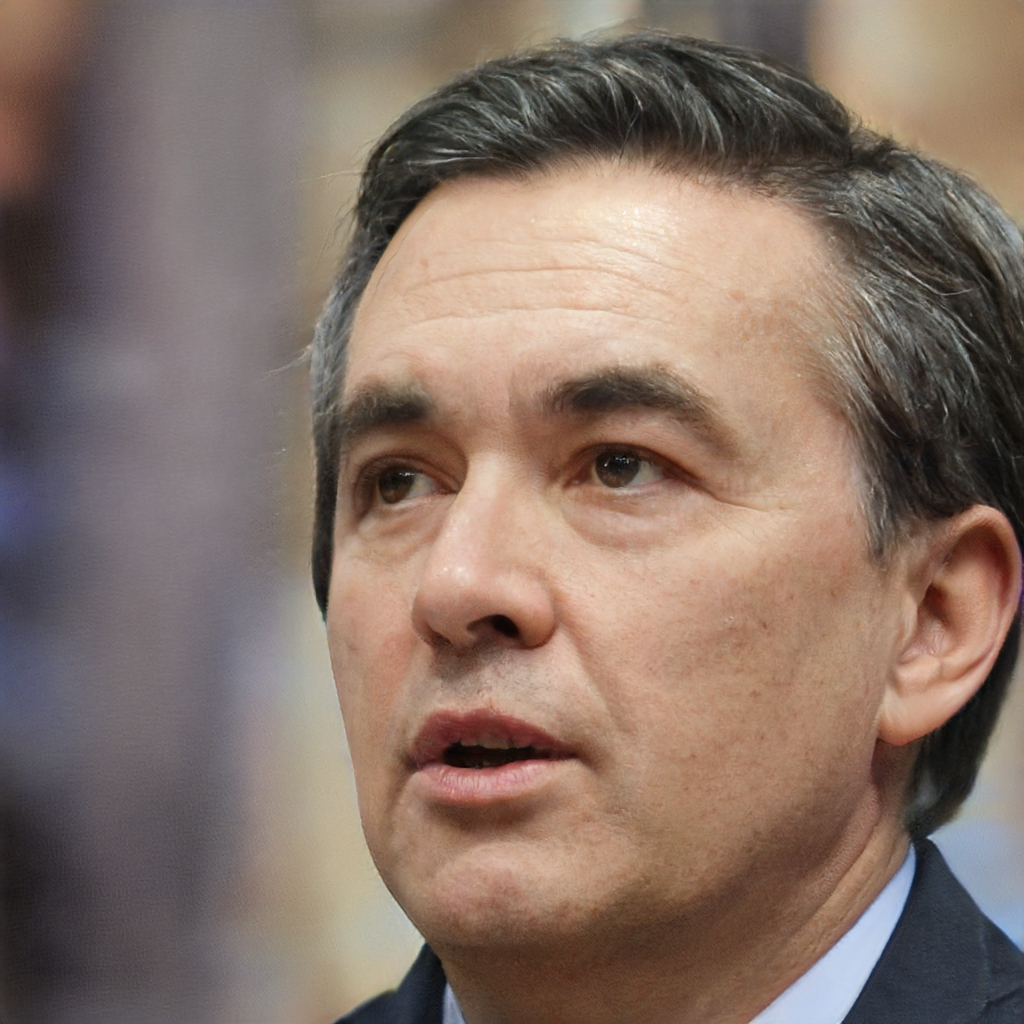
\includegraphics[width=.3\textwidth]{figures/gan-p2.jpg}}
\uncover<4->{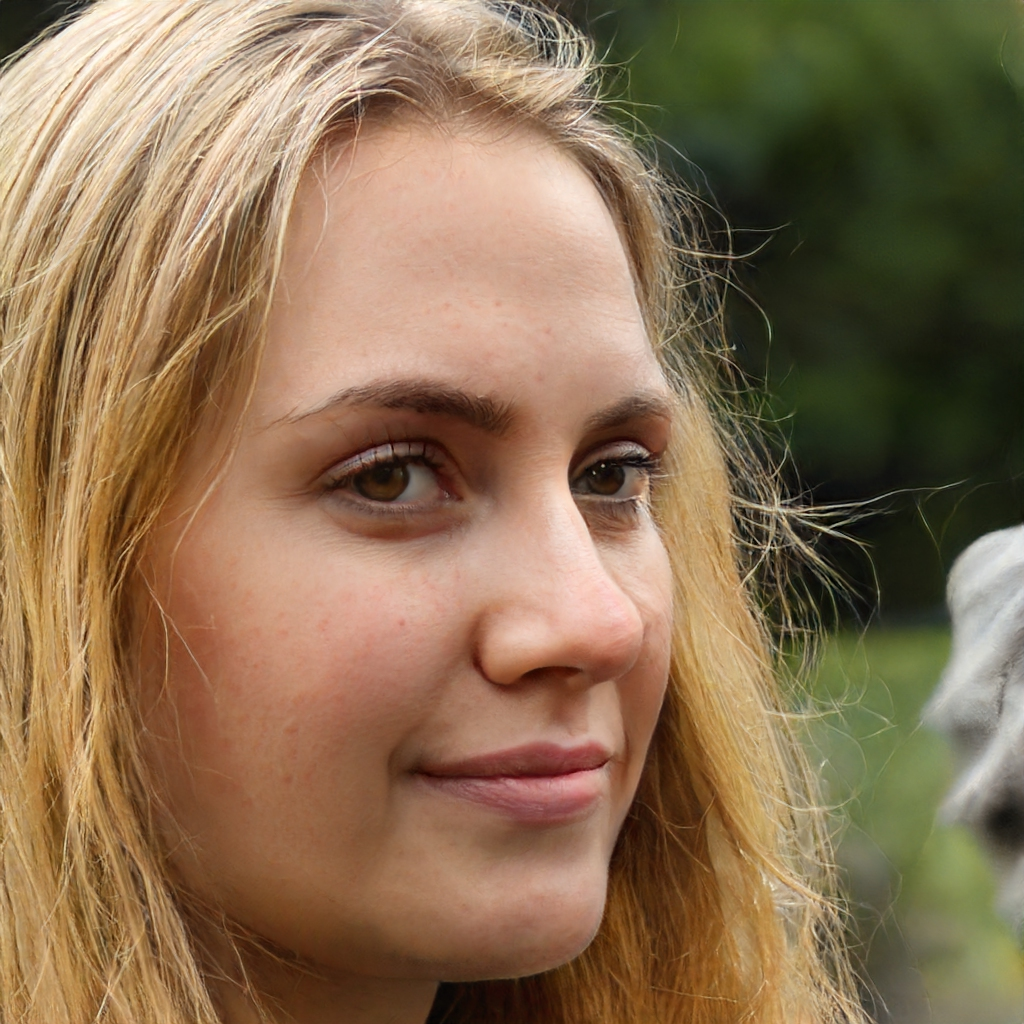
\includegraphics[width=.3\textwidth]{figures/gan-p3.jpg}}\\
\Large \uncover<5->{\color{MediumRed}None of these people are real!}
\end{center}
\end{frame}



%-----------------------------------------------
\begin{frame}{GANs}
\begin{center}

\includegraphics[width=.4\textwidth]{figures/gans.png}\\
There are hundreds(?) of different types of GANs; however, this lecture only presents the vanilla GAN. 
\end{center}
\end{frame}







%------------------------------------------------
\section{Generative Adversarial Networks}
%------------------------------------------------

%------------------------------------------------
\begin{frame}{}
\begin{center}
    \huge \bf \color{DarkBlue}
    Generative Adversarial Networks 
\end{center}
\end{frame}




%------------------------------------------------
\begin{frame}{Definitions}
    \begin{itemize}
        \item $p_{data}(\x)$: Probability distribution over the data. We assume we have access to a dataset $\{\x_i\}_{i=1}^n$; however, we do not assume we have labels nor do we need them because we're not doing classification. 
        \item<2-> $p_{g}(\zbf)$: Probability distribution over a latent variable $\zbf$. This of this distribution that is over random noise. 
        \item<3-> $G(\zbf)$: $G$ is the generator neural network that takes in a noise vector, $\zbf$, to produce a vector $\x_{fake}$. $\x_{fake}$ is a ``fake'' data sample that is generated from $\zbf$. 
        \item<4-> $D(\xbf)$: $D$ is a discriminator network that takes in a data vector $\x$ and tries to discern whether $\xbf$ was sampled from $p_{data}(\xbf)$ or generated by $G$. 
        \item<5-> Let $\theta_g$ and $\theta_d$ represent the parameters for the generator and discriminator neural networks, respectively. 
    \end{itemize}
\end{frame}

\begin{frame}{Generative Adversarial Net}
    \begin{center}
        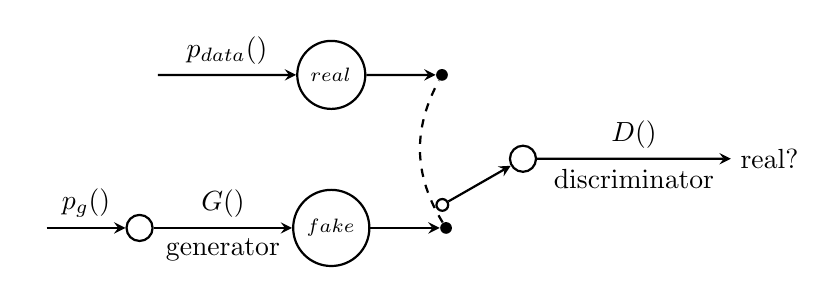
\begin{tikzpicture}[scale=0.15]
            \node[circle, draw, thick] (z) {$\zbf$};
            \node[circle, draw, thick, right=5em of z] (x) {$\x_{fake}$};
            \draw[-stealth, thick] (z) -- node[above] {$G(\zbf)$} node[below] {generator} (x);
            \node[left=of z] (i) {};
            \draw[-stealth, thick] (i) -- node[above] {$p_g(\zbf)$} (z);
            \node[above=of x, circle, draw, thick] (xt) {$\x_{real}$};
            \node[left=5em of xt] (it) {};
            \draw[-stealth, thick] (it) -- node[above] {$p_{data}(\x)$} (xt);
            \node[circle, draw, thick, right=5em of x, yshift=2.5em] (D) {$\x$};
            \node[right=7em of D] (out) {real?};
            \draw[-stealth, thick] (D) -- node[above] {$D(\x)$} node[below] {discriminator} (out);
                    
            \node[right=2.5em of x, circle, fill, inner sep=0.15em] (pt1) {};
            \node[right=2.5em of xt, circle, fill, inner sep=0.15em] (pt2) {};
                    
            \draw[dashed, thick] (pt1) edge[bend left] (pt2);
                    
            \node[circle, draw, thick, fill=white, inner sep=0.15em] at ([xshift=-0.9em, yshift=4em]pt1.north) (pt3) {};
                    
            \draw[-stealth, thick] (x) -- (pt1);
            \draw[-stealth, thick] (xt) -- (pt2);
            \draw[-stealth, thick] (pt3) -- (D);
        
        \end{tikzpicture}
        \end{center}
        
\end{frame}



%------------------------------------------------
\begin{frame}{Generative Adversarial Net}
    \small
\begin{block}{}
\begin{itemize}
    \item We have two neural network in a GAN
    \begin{itemize}
        \item The network $G$'s goal is to generate sample that look like they came from $p_{data}(\x)$. 
        \item The network $D$'s goal is to effectively discriminate between real samples from $p_{data}(\x)$ and fake samples from $G$. 
    \end{itemize}
    \item The goals of $G$ and $D$ are different! We can view this scenario as a game between $D$ and $G$. 
\end{itemize}
\end{block}


\end{frame}





%------------------------------------------------
\begin{frame}{Formally Defining the Optimization Task}

\begin{tblock}{}
The optimization of $\theta_g$ and $\theta_d$ can be cast as a $\min$-$\max$ task, which is given by
\begin{multiequation}
\min_{G}\max_{D} \left\{ \Ebb_{\xbf\sim p_{data}}\left[ \log(D(\x)) \right] + \Ebb_{\zbf\sim p_{g}}\left[\log(1 - D(G(\zbf)))\right]\right\}
\end{multiequation}
\end{tblock}


\end{frame}





%------------------------------------------------
\begin{frame}{Formally Defining the Optimization Task}
    
\begin{block}{}
\begin{itemize}
    \item If $\x \sim p_{data}(\x)$ then the discriminator should maximize $\log D(\x)$
    \item If $\zbf\sim p_g(\zbf)$ then the generator seeks to generate a sample that makes the discriminator think it is a normal sample. 
    \item We can use stochastic gradient descent and ascent to adjust the parameters of the network. 
\end{itemize}
\end{block}

\end{frame}





%------------------------------------------------
\begin{frame}{Formally Defining the Optimization Task}
\begin{alertblock}{}
Theorem 1. The global minimum of the virtual training criterion $C(G)$ is achieved if and only if $p_g = p_{data}$. At that point, $C(G)$ achieves the value $-\log (4)$. This point is a Nash Equilibrium. 
\end{alertblock}

\end{frame}




%------------------------------------------------
%------------------------------------------------
%------------------------------------------------
\begin{frame}{Pseudo Code for Training a GAN}

    \footnotesize
\begin{itemize}
    \item[ ] {\bf for} $t = 1, \ldots, T$
    \begin{itemize}
        \item[ ]  {\bf for} $k = 1, \ldots, K$
        \begin{itemize}
            \item Sample $m$ noise data $\zbf_1, \ldots, \zbf_m$ from $p_g(\zbf)$
            \item Sample $m$ data samples $\xbf_1, \ldots, \xbf_m$ from $p_{data}(\x)$
            \item  Update the discriminator by ascending its stochastic gradient:
            \begin{multiequation}
                \nabla_{\theta_d}\left\{ \frac{1}{m}\sum_{i=1}^m \left[ \log(D(\x_i)) + \log(1 - D(G(\zbf_i))) \right]\right\}
            \end{multiequation}
        \end{itemize}
        \item[ ] {\bf end for}
        \item  Sample $m$ noise data $\zbf_1, \ldots, \zbf_m$ from $p_g(\zbf)$
        \item Update the generator by descending its stochastic gradient:
        \begin{multiequation}
            \nabla_{\theta_g} \left\{  \frac{1}{m}\sum_{i=1}^m \log(1 - D(G(\zbf_i)))  \right\}
        \end{multiequation}
    \end{itemize}
    \item[ ] {\bf end for}
\end{itemize}

\end{frame}





%------------------------------------------------
\begin{frame}{Formally Defining the Optimization Task}

\begin{center}
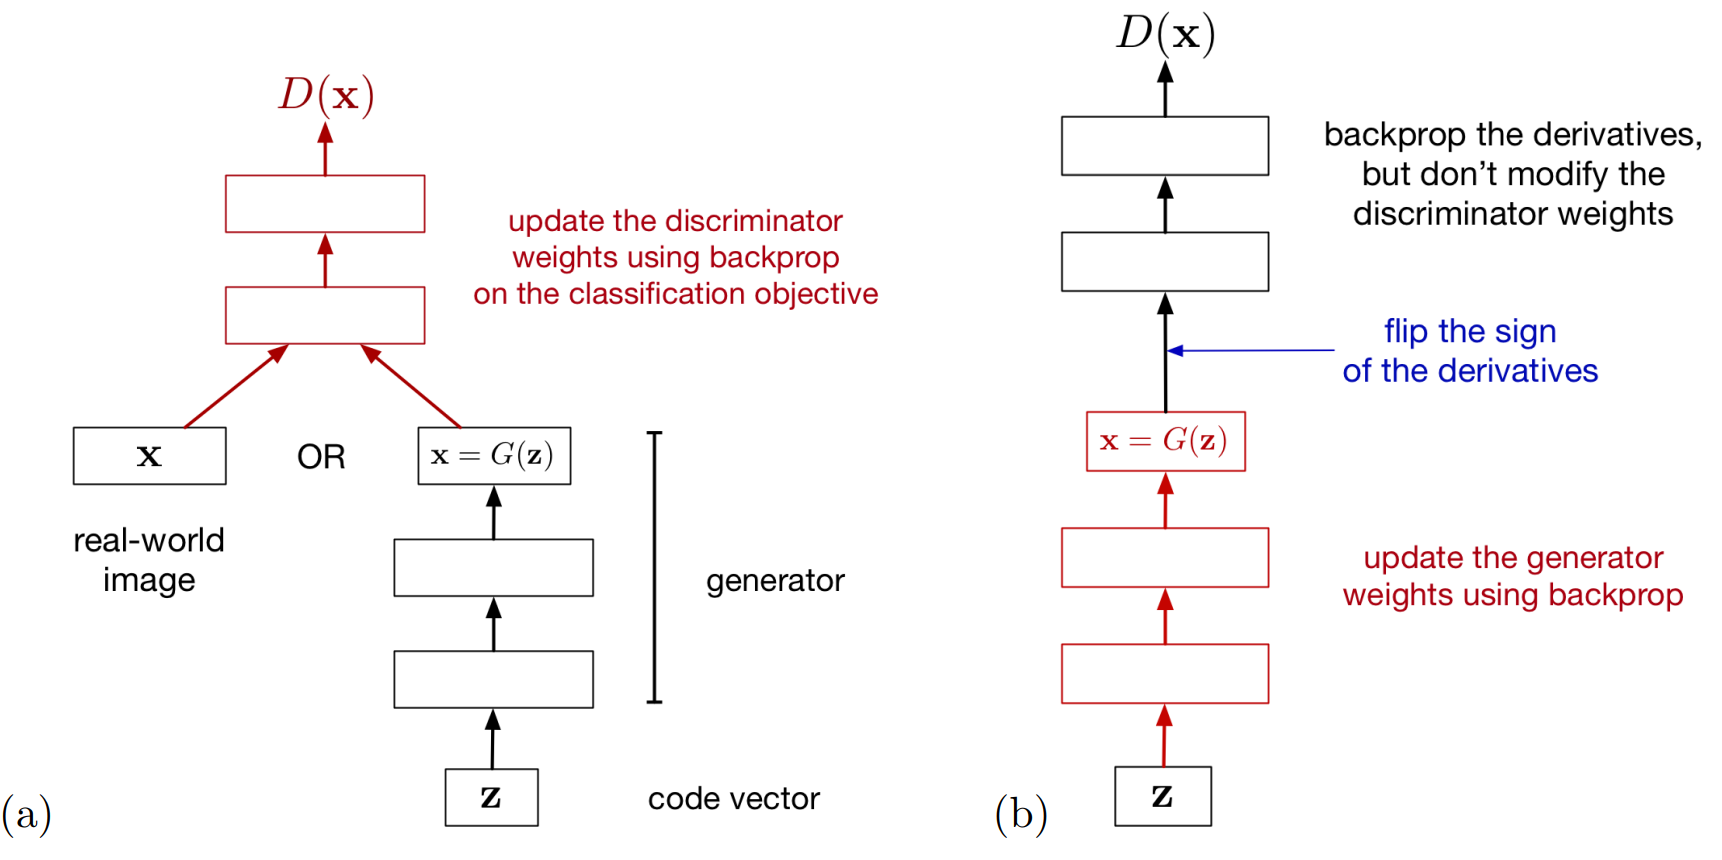
\includegraphics[height=.7\textheight]{figures/gan-opt.png}\\
From Roger Grosse's GAN lecture notes.
\end{center}

\end{frame}









%------------------------------------------------
\begin{frame}{On Training GANs}
\small

\begin{block}{Challenge}
One issue associated with training a GAN is the form of the loss. Observe above that the generator weights only get updated by the gradients of the second term:
\begin{multiequation}
\log(1 - D(G(\zbf)))
\end{multiequation}\vspace{-2em}
\begin{itemize}
    \item The problem with this is that if the generator sample is really bad, then the discriminator’s prediction is close to zero, and since $\log(1-D)$ is very flat when $D\approx0$ there is not enough ``signal'' to move the generator weights meaningfully. 
    \item Increasing learning rates do not seem to help. This is called the {\em saturation problem} in GANs. 
    \item To fix this, while updating generator weights, it is common to heuristically replace the second term in the GAN loss with $-\log D(G(\zbf))$
\end{itemize}
\end{block}


\end{frame}



%------------------------------------------------
\begin{frame}{On Training GANs}

    \small

\begin{tblock}{Challenge}
Stably training GANs was a challenge faced by the community for quite some time (and continues to be a challenge), and a common resolution is to use {\em Wasserstein GANs. }
\begin{itemize}
    \item The GAN loss is a  form of distance between probability distributions (called the Jensen-Shannon divergence), and this can be generated to other distances. 
    \item A common alternative is the Earth-mover or Wasserstein distance, leading to a different type of GAN model called Wasserstein GAN. The WGAN was shown to improve stability of the optimization process
\end{itemize}
\end{tblock}


\end{frame}




%------------------------------------------------
\begin{frame}[fragile]{GANs (in PyTorch)}

    \footnotesize

    \begin{verbatim}
class Generator(nn.Module):
    def __init__(self):
        super(Generator, self).__init__()
        def block(in_feat, out_feat, normalize=True):
            layers = [nn.Linear(in_feat, out_feat)]
            if normalize:
                layers.append(nn.BatchNorm1d(out_feat, 0.8))
            layers.append(nn.LeakyReLU(0.2, inplace=True))
            return layers
        self.model = nn.Sequential(
            *block(latent_dim, 128, normalize=False),
            *block(128, 256), *block(256, 512), *block(512, 1024),
            nn.Linear(1024, int(np.prod(img_shape))), nn.Tanh())
    def forward(self, z):
        img = self.model(z)
        img = img.view(img.size(0), *img_shape)
        return img

\end{verbatim}

\end{frame}

%------------------------------------------------
\section{GAN in PyTorch}
%------------------------------------------------

%------------------------------------------------
\begin{frame}{}
\begin{center}
    \huge \bf \color{DarkBlue}
    GAN in PyTorch 
\end{center}
\end{frame}



%------------------------------------------------
\begin{frame}[fragile]{GANs (in PyTorch)}

    \footnotesize

    \begin{verbatim}
class Discriminator(nn.Module):
    def __init__(self):
        super(Discriminator, self).__init__()
        self.model = nn.Sequential(
            nn.Linear(int(np.prod(img_shape)), 512),
            nn.LeakyReLU(0.2, inplace=True),
            nn.Linear(512, 256),
            nn.LeakyReLU(0.2, inplace=True),
            nn.Linear(256, 1),
            nn.Sigmoid(),
        )
    def forward(self, img):
        img_flat = img.view(img.size(0), -1)
        validity = self.model(img_flat)
        return validity
\end{verbatim}

\end{frame}




%------------------------------------------------
\begin{frame}[fragile]{GANs (in PyTorch)}
\tiny
\begin{verbatim}
for epoch in range(n_epochs):
    for i, (imgs, _) in enumerate(dataloader):
        # Adversarial ground truths
        valid = Variable(Tensor(imgs.size(0), 1).fill_(1.0), requires_grad=False)
        fake = Variable(Tensor(imgs.size(0), 1).fill_(0.0), requires_grad=False)
        # Configure input
        real_imgs = Variable(imgs.type(Tensor))
        # -----------------
        #  Train Generator
        optimizer_G.zero_grad()
        # Sample noise as generator input
        z = Variable(Tensor(np.random.normal(0, 1, (imgs.shape[0], latent_dim))))
        # Generate a batch of images
        gen_imgs = generator(z)
        # Loss measures generator's ability to fool the discriminator
        g_loss = adversarial_loss(discriminator(gen_imgs), valid)
        g_loss.backward()
        optimizer_G.step()
        # ---------------------
        #  Train Discriminator
        optimizer_D.zero_grad()
        # Measure discriminator's ability to classify real from generated samples
        real_loss = adversarial_loss(discriminator(real_imgs), valid)
        fake_loss = adversarial_loss(discriminator(gen_imgs.detach()), fake)
        d_loss = (real_loss + fake_loss) / 2
        d_loss.backward()
        optimizer_D.step()
\end{verbatim}

\end{frame}




%------------------------------------------------
\begin{frame}{GAN Loss}
\begin{center}
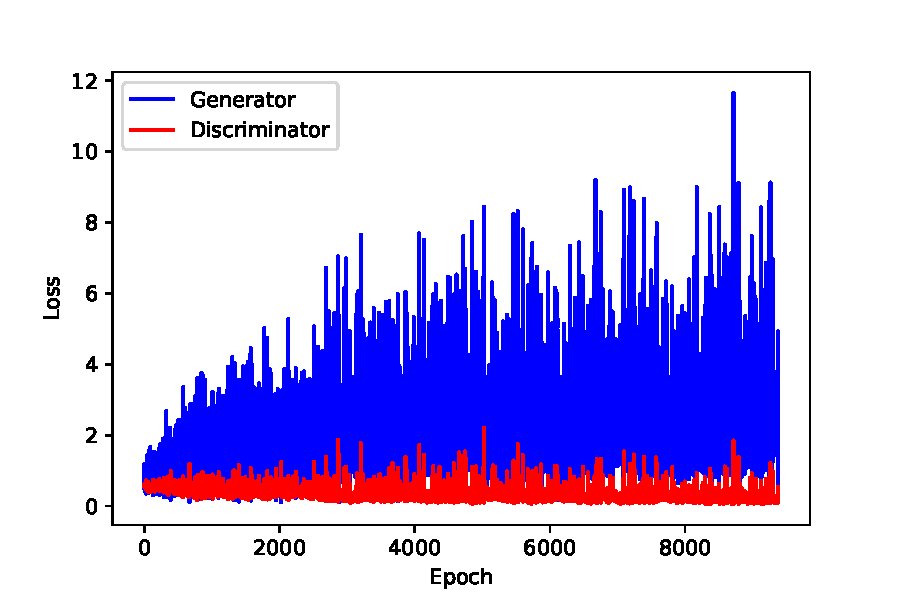
\includegraphics[width=.7\textwidth]{figures/gan-losses.pdf}
\end{center}
\end{frame}




%------------------------------------------------
\section{Examples}
%------------------------------------------------

%------------------------------------------------
\begin{frame}{}
\begin{center}
    \huge \bf \color{DarkBlue}
    Examples 
\end{center}
\end{frame}




%------------------------------------------------
%------------------------------------------------



%------------------------------------------------
\begin{frame}{GAN example}
\begin{center}
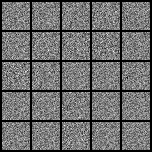
\includegraphics[width=.3\textwidth]{figures/gan-mnist-0.png}
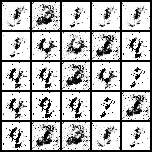
\includegraphics[width=.3\textwidth]{figures/gan-mnist-400.png}
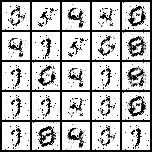
\includegraphics[width=.3\textwidth]{figures/gan-mnist-8000.png}
\end{center}
\end{frame}


%------------------------------------------------
\begin{frame}{GAN example: Sketch to Figure}
\begin{center}
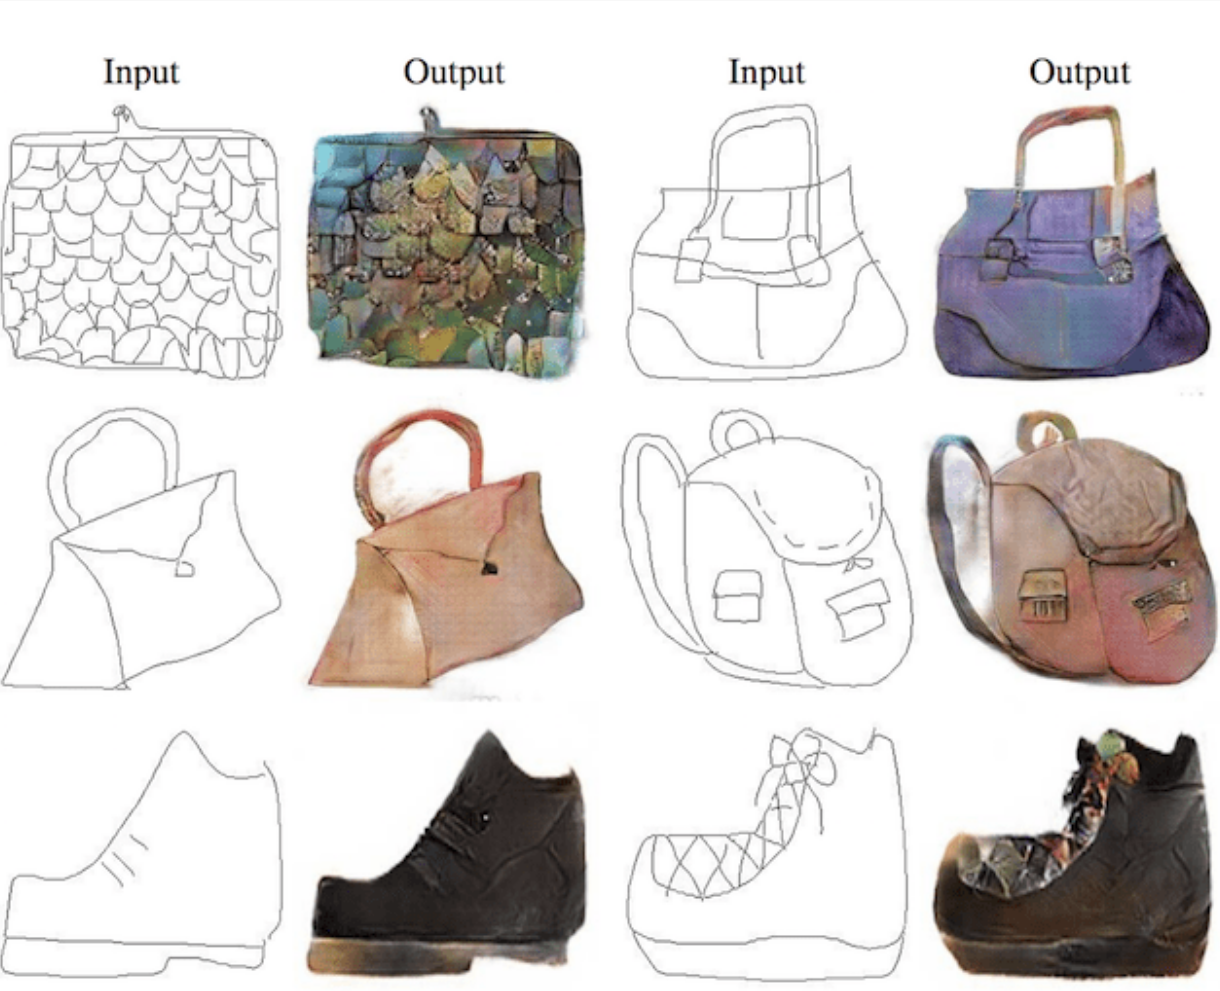
\includegraphics[width=.6\textwidth]{figures/gan-sketch.png}
\end{center}
\end{frame}


%------------------------------------------------
\begin{frame}{GAN example: Cycle GANs}

\begin{block}{}
\begin{itemize}
\item Image-to-image translation involves generating a new synthetic version of a given image with a specific modification, such as translating a summer landscape to winter
\end{itemize}
\end{block}

\end{frame}



%------------------------------------------------
\begin{frame}{GAN example: Cycle GANs}
\begin{center}
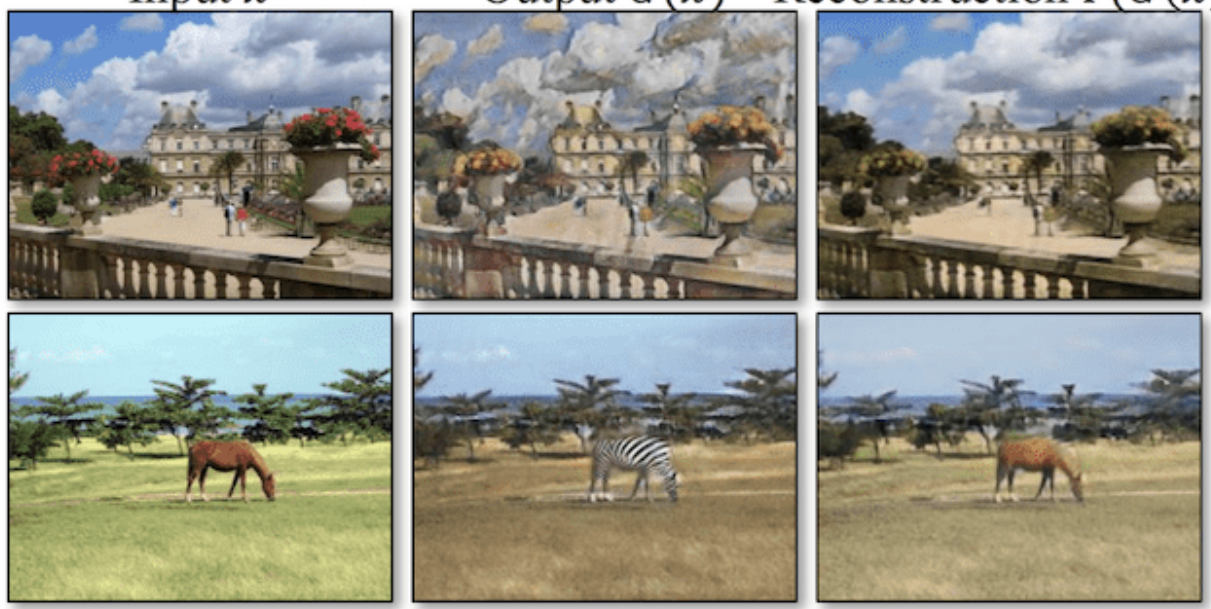
\includegraphics[width=.8\textwidth]{figures/gan-style.png}
\end{center}
\end{frame}


%------------------------------------------------
\begin{frame}{GAN example: Cycle GANs}
\begin{center}
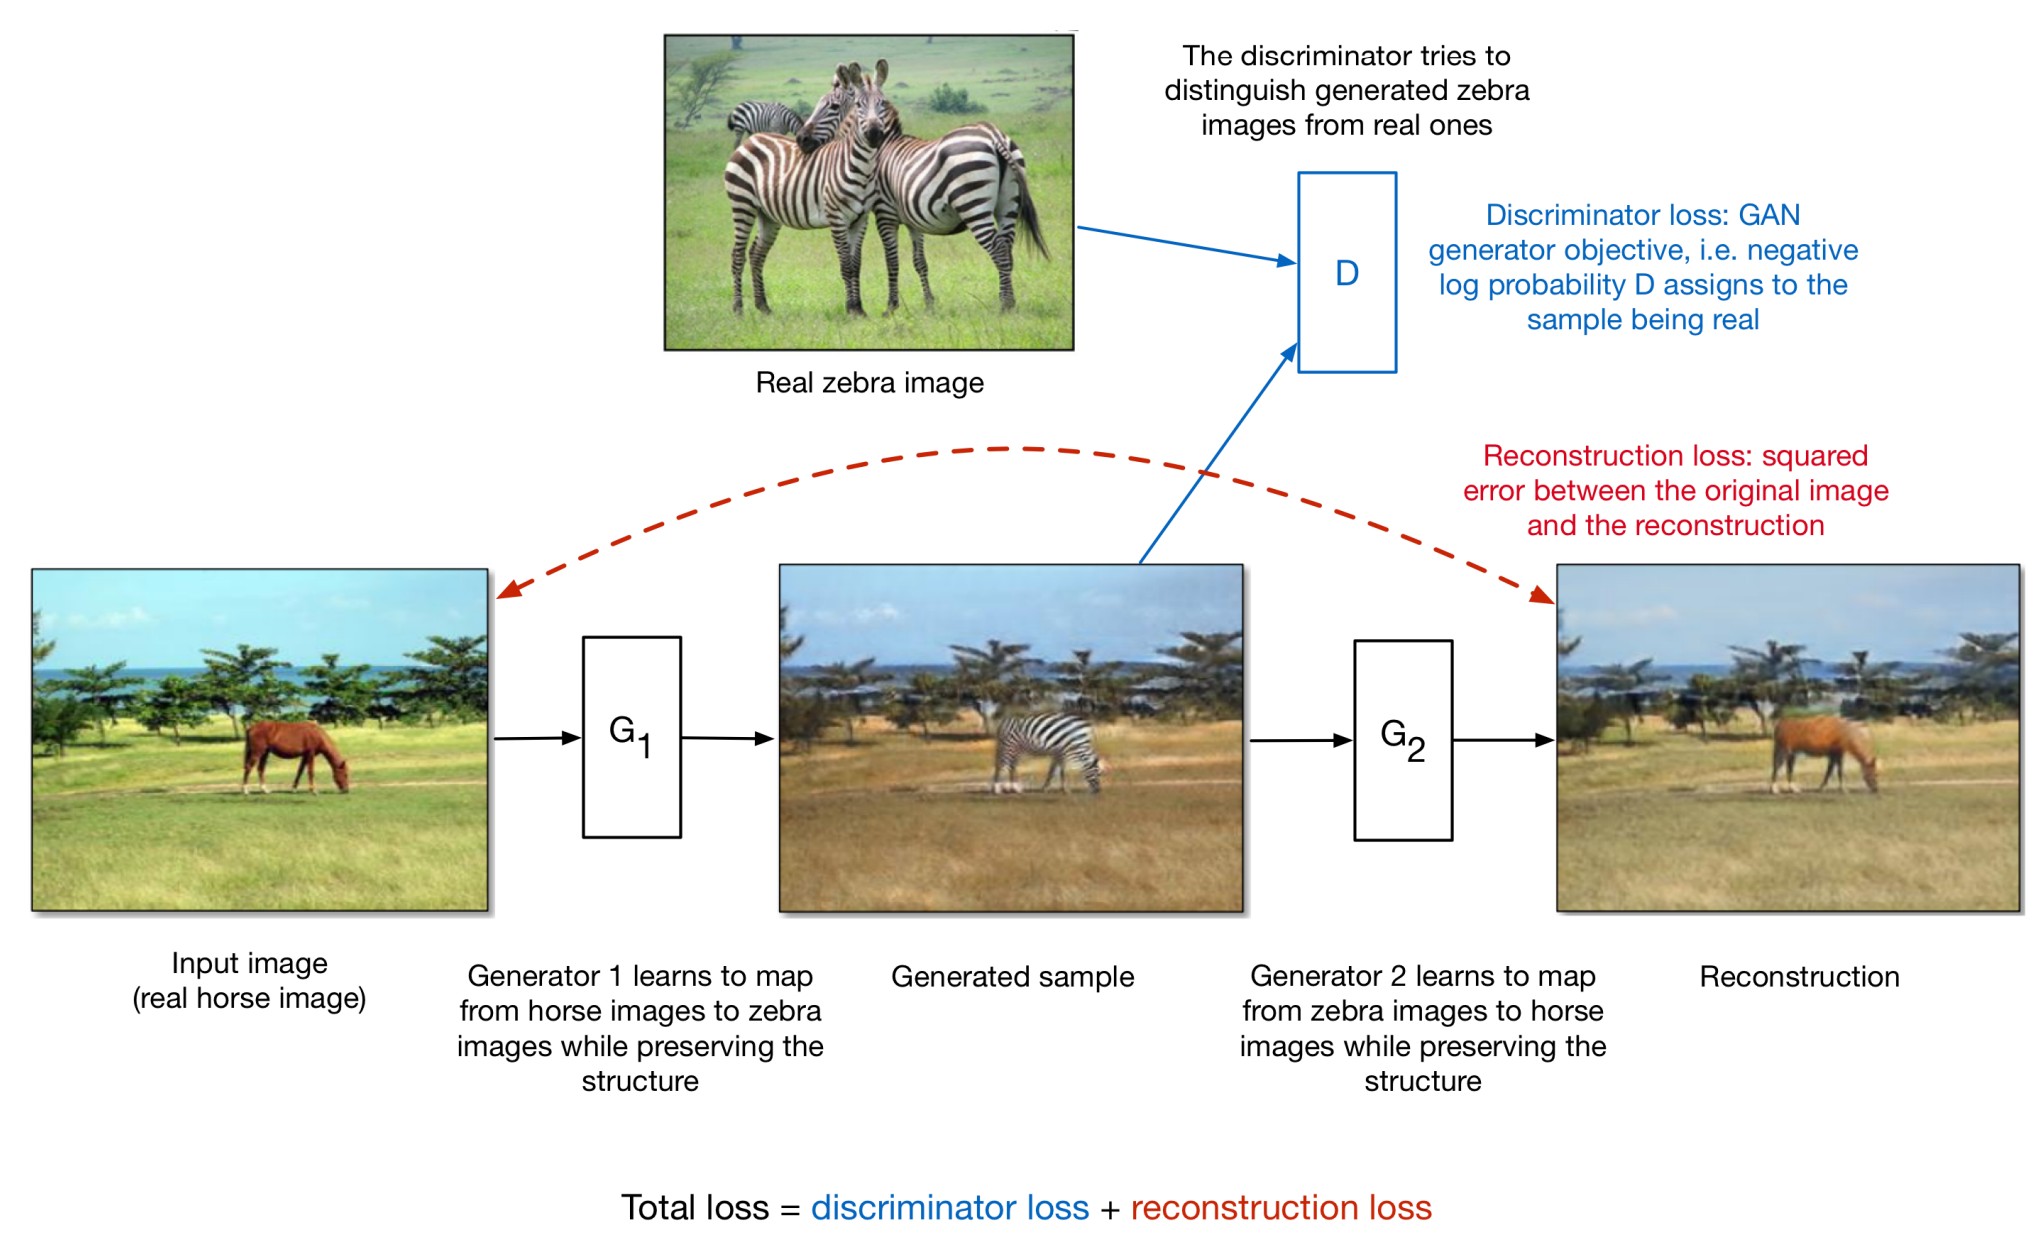
\includegraphics[width=.8\textwidth]{figures/gan-cycle.png}
\end{center}
\end{frame}



%------------------------------------------------
% \begin{frame}{First AI-Generated Portrait Ever Sold at Auction Shatters Expectations}
% \begin{center}
% \uncover<2->{
\includegraphics[width=.6\textwidth]{figures/gan-arrested.jpg}}
% \end{center}
% \end{frame}


%------------------------------------------------
\begin{frame}{First AI-Generated Portrait Ever Sold at Auction Shatters Expectations: \$432,500}
\begin{center}
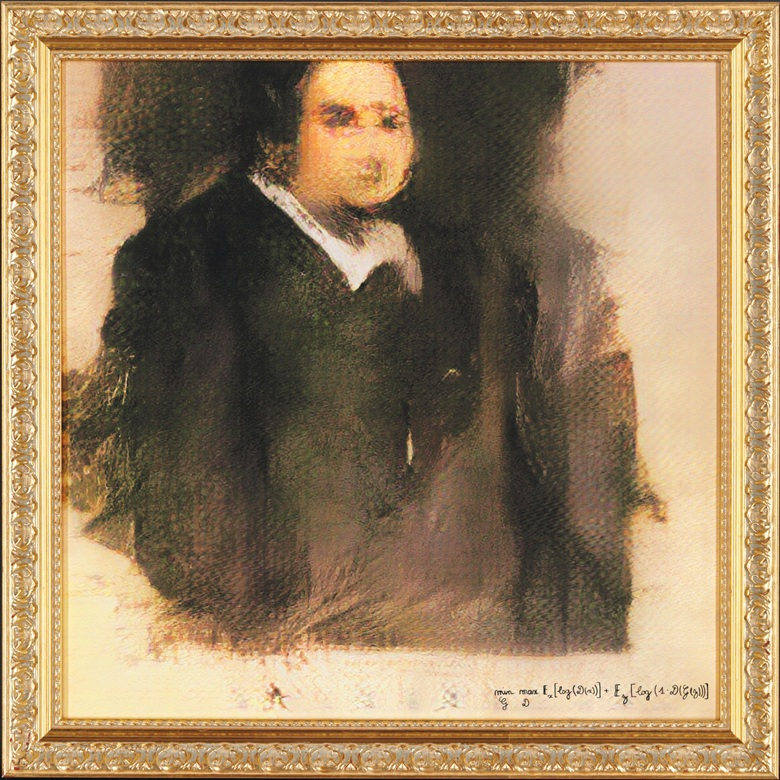
\includegraphics[width=.4\textwidth]{figures/gan-art.jpg}
\end{center}
\end{frame}


%------------------------------------------------
\begin{frame}{Cosmopolitan Meets DALL-E 2} 
\begin{center}
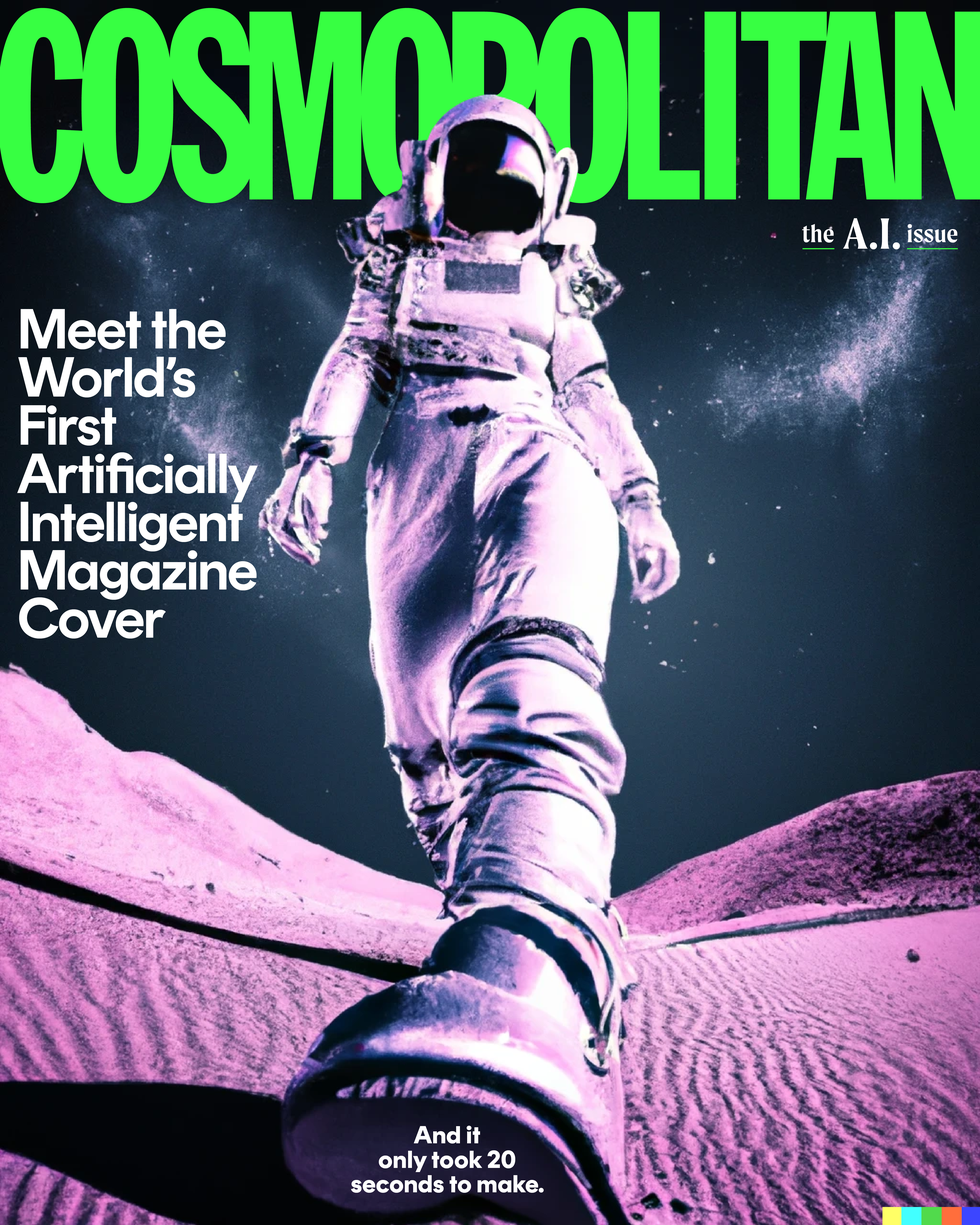
\includegraphics[width=.4\textwidth]{figures/gan-cosmo.png}
\end{center}
\end{frame}



%------------------------------------------------
\begin{frame}{DALL-E 2: Text-to-Image Synthesis}

\begin{block}{}
\begin{itemize}
\item DALL-E 2 is a new AI system that can create realistic images and art from a description in natural language.
DALL-E 2 can create original, realistic images and art from a text description. It can combine concepts, attributes, and styles.
% DALL-E's model is a multimodal implementation of GPT-3[16] with 12 billion parameters[1] which "swaps text for pixels", trained on text-image pairs from the Internet.[17] DALL-E 2 uses 3.5 billion parameters, a smaller number than its predecessor
\item DALL-E's uses multimodal version of GPT-3 with 12 billion parameters. The concept is that it swaps text for pixels and it is trained on trained on text-image pairs from the Internet. DALL-E 2 uses 3.5 billion parameters. 
\end{itemize}
\end{block}

\end{frame}



%------------------------------------------------
\begin{frame}{DALL-E 2} 
\begin{center}
``a painting of a fox sitting
in a field at sunrise in the
style of Claude Monet''\\
\uncover<2->{
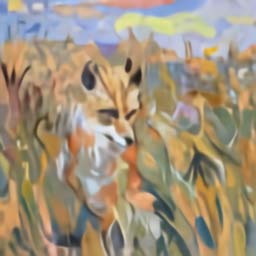
\includegraphics[width=.4\textwidth]{figures/dall-e-1.jpg}
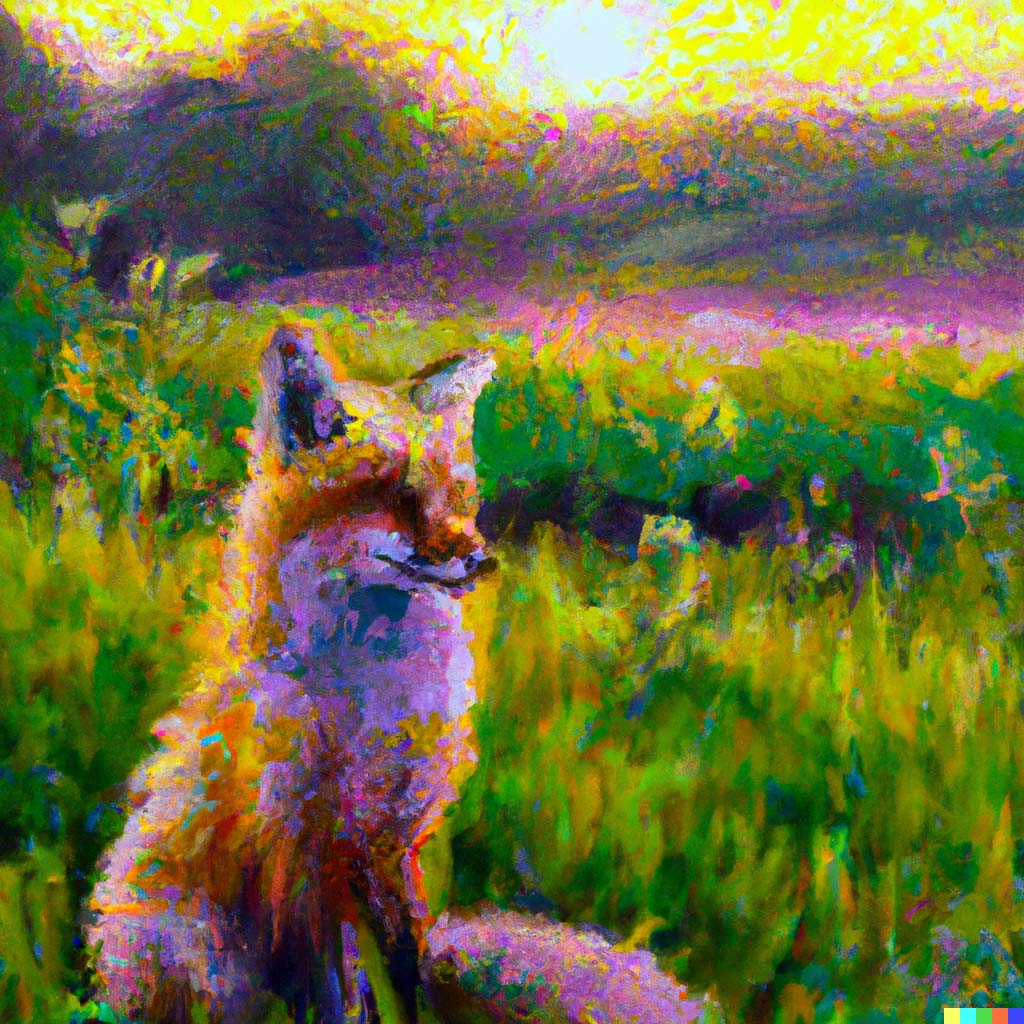
\includegraphics[width=.4\textwidth]{figures/dall-e-2.jpg}
}
\end{center}
\end{frame}












%------------------------------------------------
\section{Challenges with GANs}
%------------------------------------------------

%------------------------------------------------
\begin{frame}{}
\begin{center}
    \huge \bf \color{DarkBlue}
    Challenges with GANs 
\end{center}
\end{frame}





%------------------------------------------------

\begin{frame}{Issues with GANs (Google's Comments)}
\begin{tblock}{}
\begin{itemize}
    \item Research has suggested that if your discriminator is too good, then generator training can fail due to vanishing gradients. In effect, an optimal discriminator doesn't provide enough information for the generator to make progress.
    \begin{itemize}
        \item The Wasserstein loss is designed to prevent vanishing gradients even when you train the discriminator to optimality. 
    \end{itemize}
    \item The generator may learn to produce a single output. The generator is always trying to find the one output that seems most plausible to the discriminator. This form of GAN failure is called {\em mode collapse}.
    \item GANs frequently fail to converge, as discussed in the module on training.
\end{itemize}
\end{tblock}
\end{frame}





%------------------------------------------------
% \begin{frame}{Wasserstein GAN}
% \begin{tblock}{}
% \begin{multiequation}
    
% \end{multiequation}
% \end{tblock}
% \end{frame}

%------------------------------------------------
%------------------------------------------------
%------------------------------------------------
%------------------------------------------------





\begin{frame}{References}
    % Beamer does not support BibTeX so references must be inserted manually as below
    \footnotesize{
        \begin{thebibliography}{99}
            \bibitem[Goodfellow, 2013]{p1} Ian J. Goodfellow, Jean Pouget-Abadie, Mehdi Mirza, Bing Xu, David Warde-Farley, Sherjil Ozair, Aaron Courville, Yoshua Bengio (2013)
            \newblock Generative Adversarial Networks
            \newblock \emph{Advances in Neural Information Processing Systems}.
        \end{thebibliography}
    }
\end{frame}




    %------------------------------------------------
    \begin{frame}
        \Huge{\centerline{\color{MediumBlue}\textbf{The End}}}
    \end{frame}

\end{document}